% Name: Uniform circular motion
% Description: A body moving at constant speed on a circle of radius r: its velocity along the tangent, its centripetal acceleration toward the center, and the angular speed ω.
% Tags: circular motion, centripetal acceleration, angular velocity, kinematics

\usetikzlibrary{arrows.meta}

\begin{tikzpicture}[>={Stealth[length=2.5mm]}, every node/.style={font=\small}]
  \coordinate (O) at (0,0);
  \coordinate (P) at (35:2.4);
  \draw[thick, gray] (O) circle (2.4);
  \fill (O) circle (1.5pt) node[below left] {$O$};
  \draw[thick] (O) -- node[pos=0.35, below right] {$r$} (P);
  % The velocity is along the tangent (35 + 90 = 125 degrees); the acceleration points back along the radius.
  \draw[->, very thick, red!70!black] (P) -- ++(125:1.6) node[above] {$\vec{v}$};
  \draw[->, very thick, blue!70!black] (P) -- ++(215:1.1) node[above left=-1pt] {$\vec{a}_c$};
  \draw[->, thick, gray!40!black] (60:0.7) arc[start angle=60, end angle=150, radius=0.7] node[left] {$\omega$};
  \fill[orange!80!black] (P) circle (3.5pt);
  \node[anchor=west, align=left] at (3.1,-0.6) {$v = \omega r$\\[2pt] $a_c = \dfrac{v^2}{r} = \omega^2 r$};
\end{tikzpicture}
